\documentclass{article}
\usepackage[utf8]{inputenc}
\usepackage{amssymb}
\usepackage{changepage}
\usepackage{graphicx}
\usepackage[backend=bibtex,
style=numeric
%style=alphabetic
%style=reading
]{biblatex}
\addbibresource{sources}

\title{Predicting New Contracts in NBA Free Agency}
\begin{document}
\author{Calvin Szeto}
\maketitle
\section{Introduction}

\subsection{Motivation}

The goal of this project is to find meaningful relationships between player performance data and the salaries they earn. These relationships provide opportunities for basketball fans and professionals to enhance their understanding of the NBA player market. For a fan, the visualizations provide insight into whether their favorite players are truly overpaid or underpaid. For a professional, the models allow them to predict the market for certain players in certain years, and they can adjust their contract negotiations accordingly.

\subsection{Problem}

Prediction of salaries is a non-trivial problem. The amount a player is paid depends on a large number of features, not only performance and skill data, but also personality, athleticism, and the current market. Further, performance data such as box scores and even advanced statistics are still not completely representative of a player's true skillset. Nevertheless, there is enough meaningful substance in available data to cluster similar players together, and from these clusters perhaps find a reasonable estimate of the market for a certain type of player. 

\subsection{Data and Algorithms}

To satisfy this goal, multiple algorithms are applied to scraped data and compared side-by-side. These algorithms include k-Means using both the Lloyd-Forgy method and Hartigan-Wong method, Spectral Clustering based on a k-Nearest-Neighbors graph, and k-Means with Principal Component Analysis. These clustering algorithms allow us to cluster players meaningfully, and to examine salary statistics for individual clusters.

The data used includes regular box score data and advanced statistics downloaded from Basketball-Reference \cite{brseason}, salary data scraped from Basketball-Reference \cite{brplayers}, and free agency lists scraped from Wikipedia \cite{wikipedia}. These datasets are joined to relate a player's performance in a given season with their salary, and free agency data is used to identify persons of interest.

\section{Implementation}

\subsection{$k$-Means}

First, the forementioned box score data was clustered using the $k$-Means algorithm with the intention of clustering players by skillset and quality of performance.

To begin, the version of $k$-means commonly known as the Lloyd-Forgy method was implemented in R and applied to per-game datasets. The algorithm chooses an initial set of centroids at random, although each feature of the centers are kept within the bounds of the maximum and minimum values of the corresponding feature in the actual dataset, so as not to create unusually random centroids. An interesting problem initially encountered was the occurence of empty clusters early in the execution of the algorithm; this was easily resolved by moving a random point into each of the empty clusters. The algorithm converges quickly afterwards. A perhaps better implementation would be to choose the point with the highest error and move that into the empty cluster instead. This approach would be more data-driven and help separate clusters which are less dense.

The algorithm was run with several different values of $k$. The squared-sum-of-errors of some of these attempts are plotted here.

\begin{figure}[h!]
    \centering
    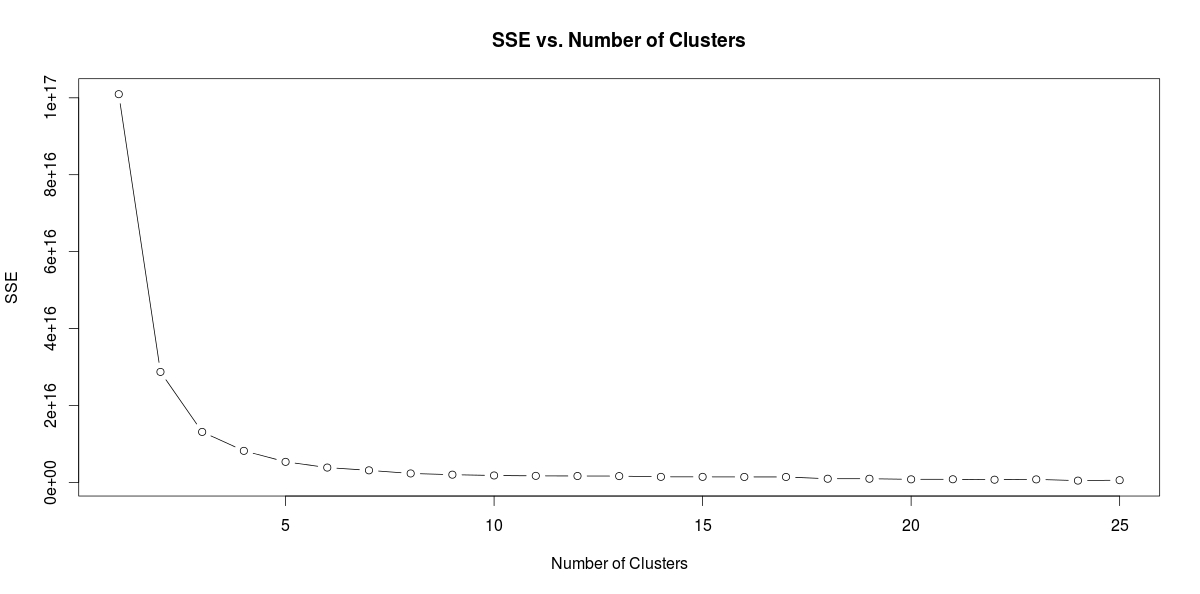
\includegraphics[width=0.8\textwidth]{sse.jpeg}
    \caption{Finding an optimal number of clusters using an SSE graph.}
\end{figure}

As expected the SSE descreases sharply within the first few clusters, and slowly afterwards. In addition to examining the errors, however, we also browse the clusters manually in hopes of finding a clustering which divides players sensibly among positions, skillsets, and quality. From such manual investigation, we find that 10-15 clusters is the sweetspot for meaningful groups.

\begin{figure}[h!]
    \centering
    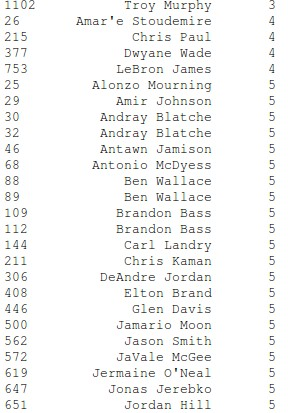
\includegraphics[scale=0.5]{sensicalcluster.jpeg}
    \caption{A sample of players ordered by cluster.}
\end{figure}

With the number of clusters decided and the algorithm converging smoothly, we run an instance of $k$-means on the dataset and merge it back with the salary data. We now have a dataset of player per-game statistics separated by season, joined with the salaries and cluster assignments.

\begin{figure}[h!]
    \centering
    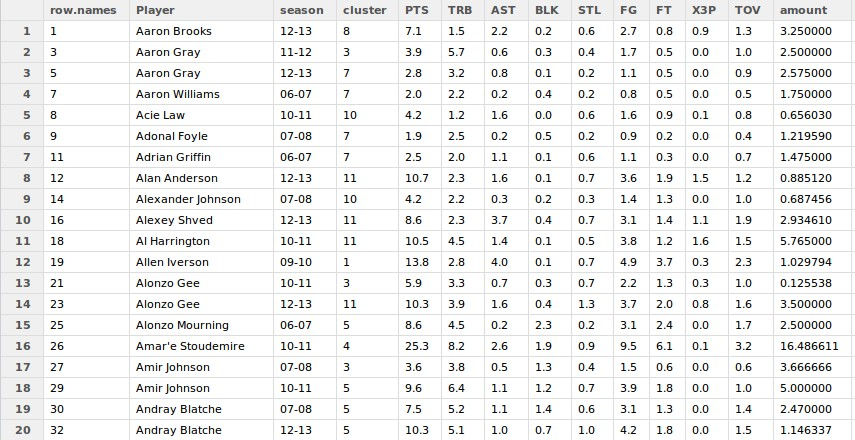
\includegraphics[width=0.8\textwidth]{sampledata.jpeg}
    \caption{A sample of the clustered dataset with a salary feature.}
\end{figure}

Finally, we are particularly interested in free agents, so we trim the current dataset to only include player seasons where the player is fresh off a new contract from free agency. This allows us to examine the type of pay players from different clusters receive on average, and to also observe players who were particularly overpaid or underpaid in the past compared to the norm.

\begin{figure}[h!]
    \centering
    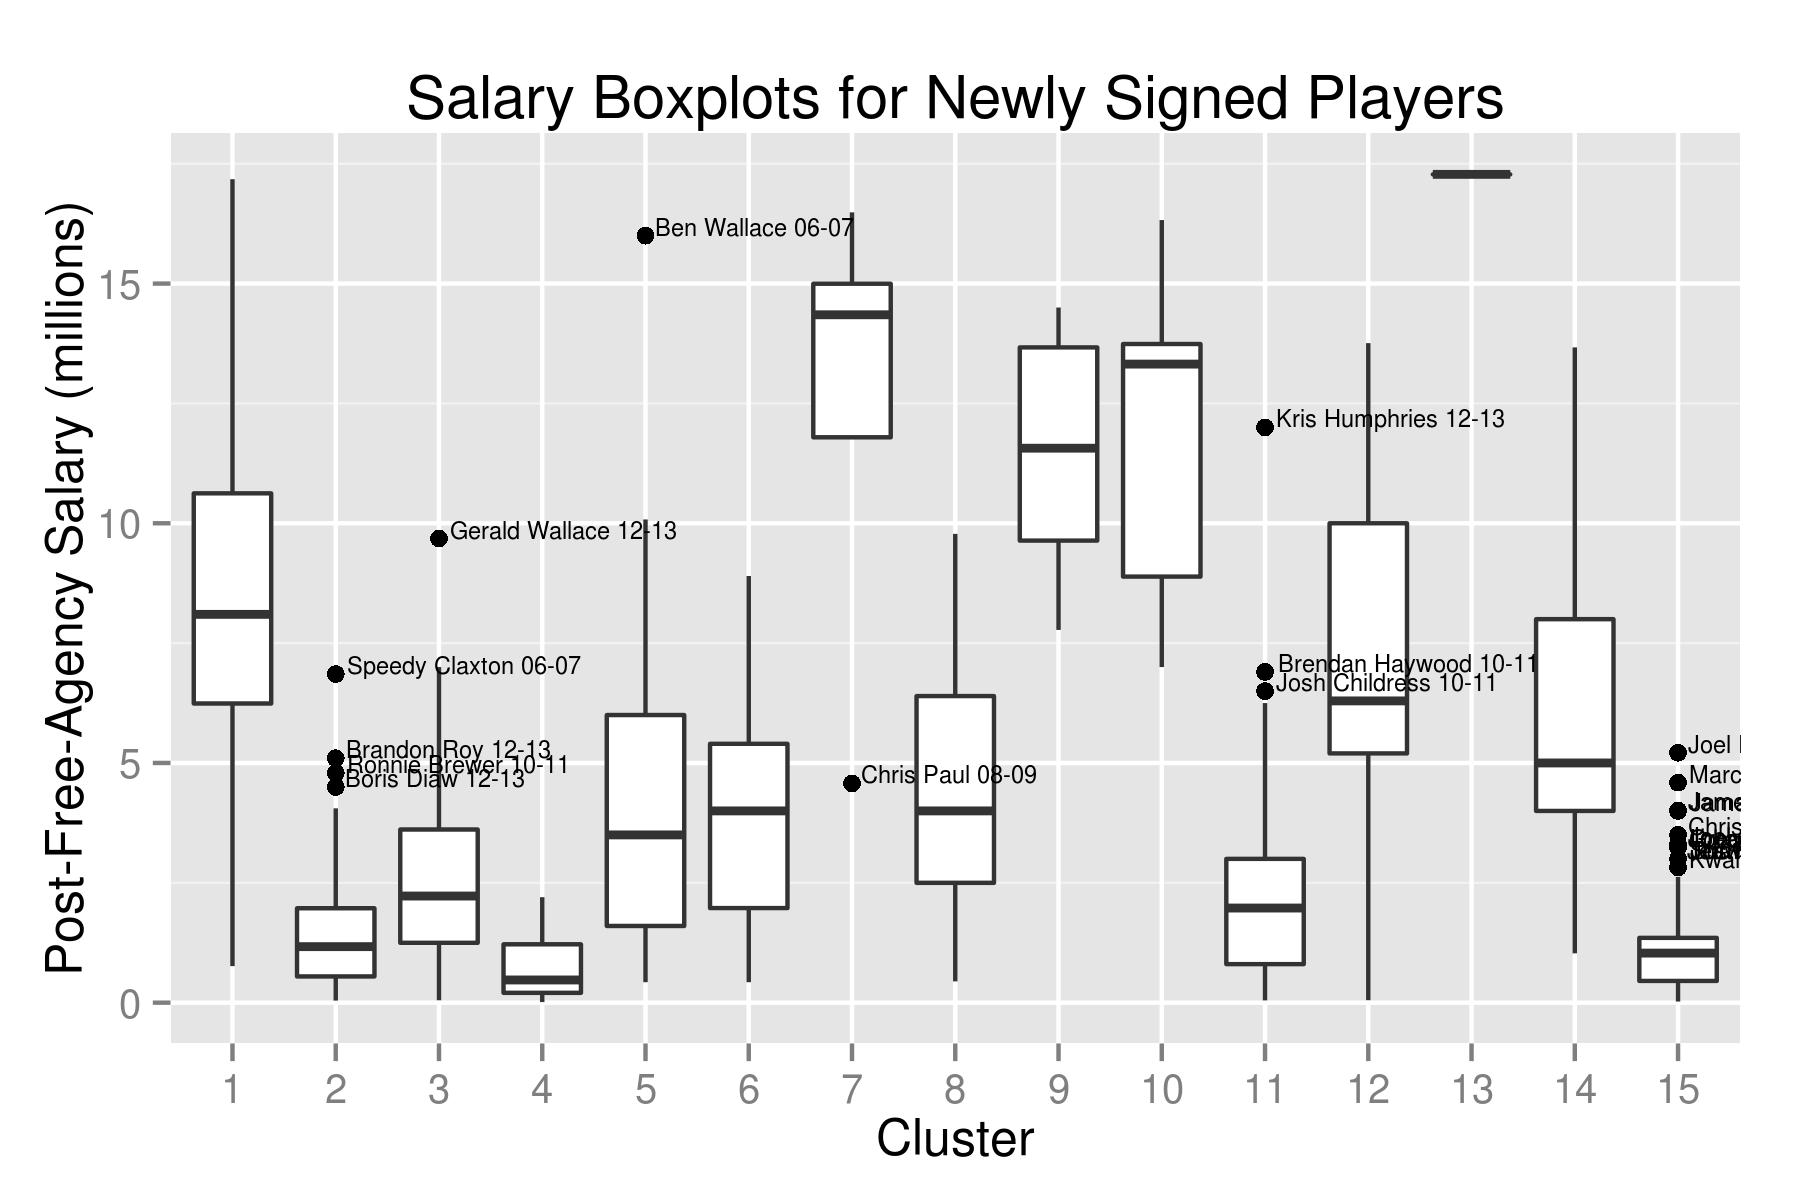
\includegraphics[width=0.8\textwidth]{lf-kmeans.jpeg}
    \caption{$k$-Means using the Lloyd-Forgy method.}
\end{figure}

In addition to the Lloyd-Forgy algorithm, another popular version of $k$-means is the Hartigan-Wong method. This method gives us similar results:

\begin{figure}[h!]
    \centering
    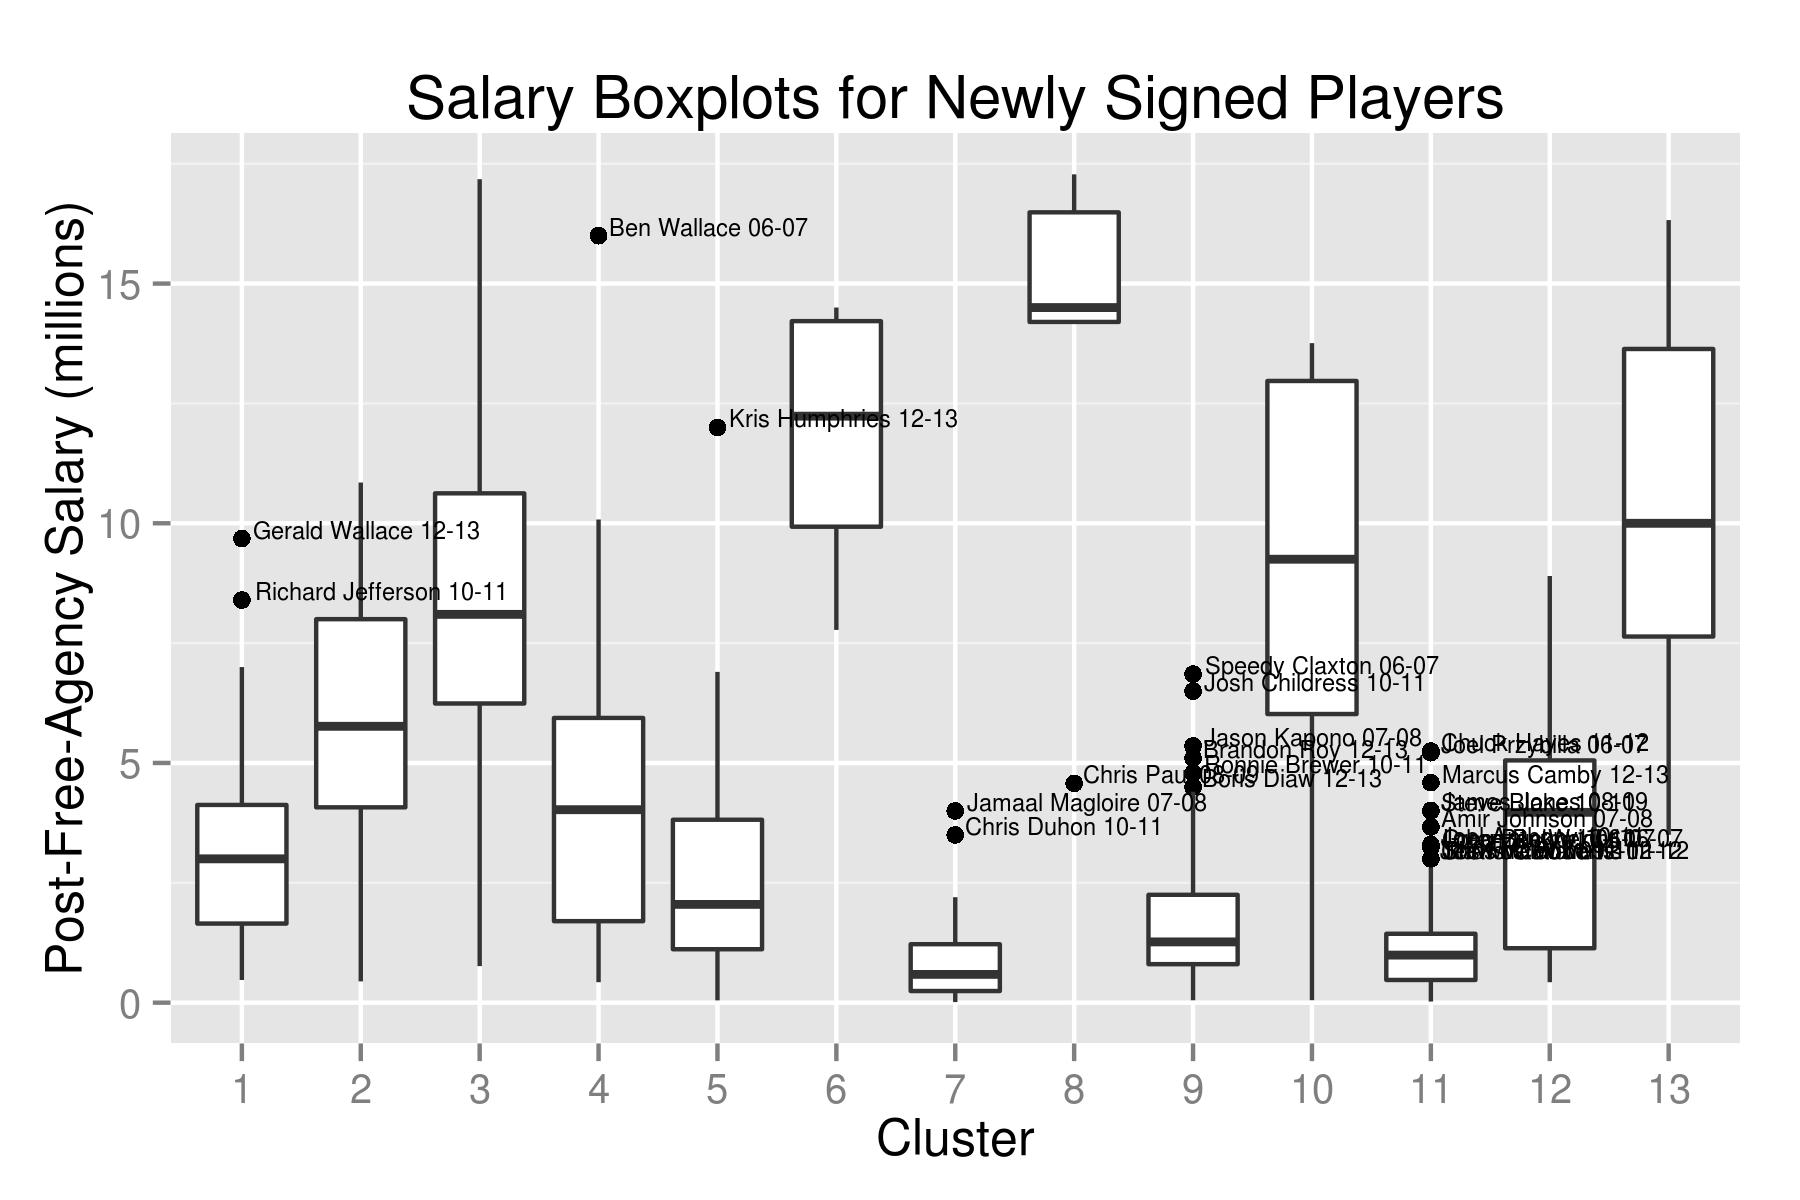
\includegraphics[width=0.8\textwidth]{hw-kmeans.jpeg}
    \caption{$k$-Means using the Hartigan-Wong method.}
\end{figure}

A major difference of Hartigan-Wong is the performance - compared to our implementation of the Lloyd-Forgy algorithm, the Hartigan-Wong implementation in the R libraries runs considerably faster. Note that every run of $k$-Means gives similar but different results - since we intitialize our centroids randomly, the algorithm will converge on different centroids on every execution.

\subsection{$k$-Nearest-Neighbors}

Another common clustering algoritm is a modification of the common classification algorithm, $k$-Nearest-Neighbors. This clustering algorithm has a few advantages - most importantly, it benefits from data which is not necessarily meaningful using Euclidean distance, as $k$-Means does.

\begin{figure}[h!]
    \centering
    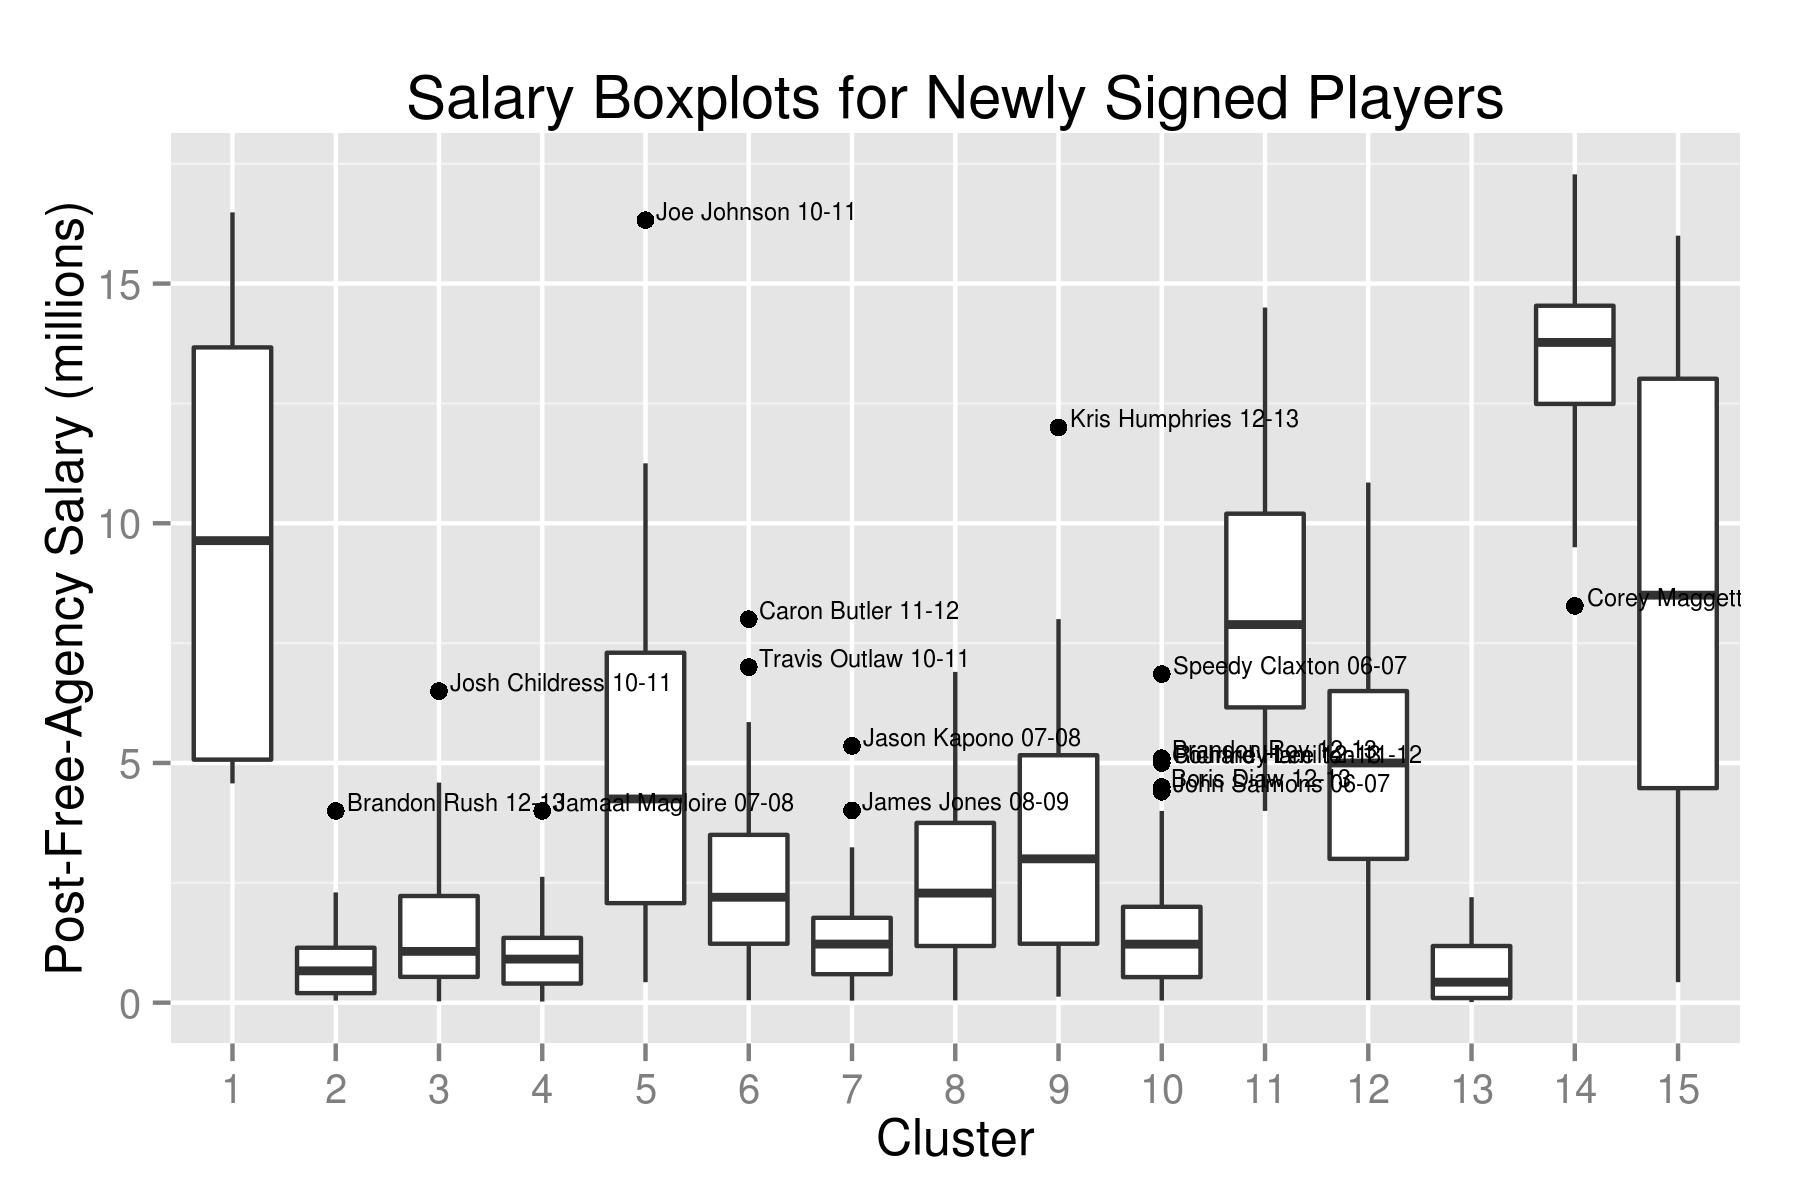
\includegraphics[width=0.8\textwidth]{sc.jpeg}
    \caption{Spectral Clustering using a $k$-Nearest-Neighbors graph.}
\end{figure}

Here, we use Spectral Clustering based on a $k$-Nearest-Neighbors graph for similarity. Spectral Clustering calculates the eigenvectors of the data before clustering in order to reduce the dimensions - see the Principal Component Analysis subsection for more.

\subsection{Principal Component Analysis}

An issue which is common among machine learning situations is high-dimensional data. Most data is naturally multidimensional - for example, the simple box score data already has at least 9 major features, as well as other possibly important features such as age, games played, etc. Multidimensional data is difficult to reason with intuitively, and can introduce a lot of noise. One common method to reduce the number of dimensions is Principal Component Analysis, which decomposes the data matrix into eigenvectors and sorts them based on eigenvalues. The resulting vectors happen to be sorted by the amount of variance which they account for, with the highest eigenvectors tending to account for a large percentage of the total variance.

We use this method to our advantage by running PCA on the players dataset and running $k$-Means as before using the first two major eigenvectors as the input. The results are very similar:

\begin{figure}[h!]
    \centering
    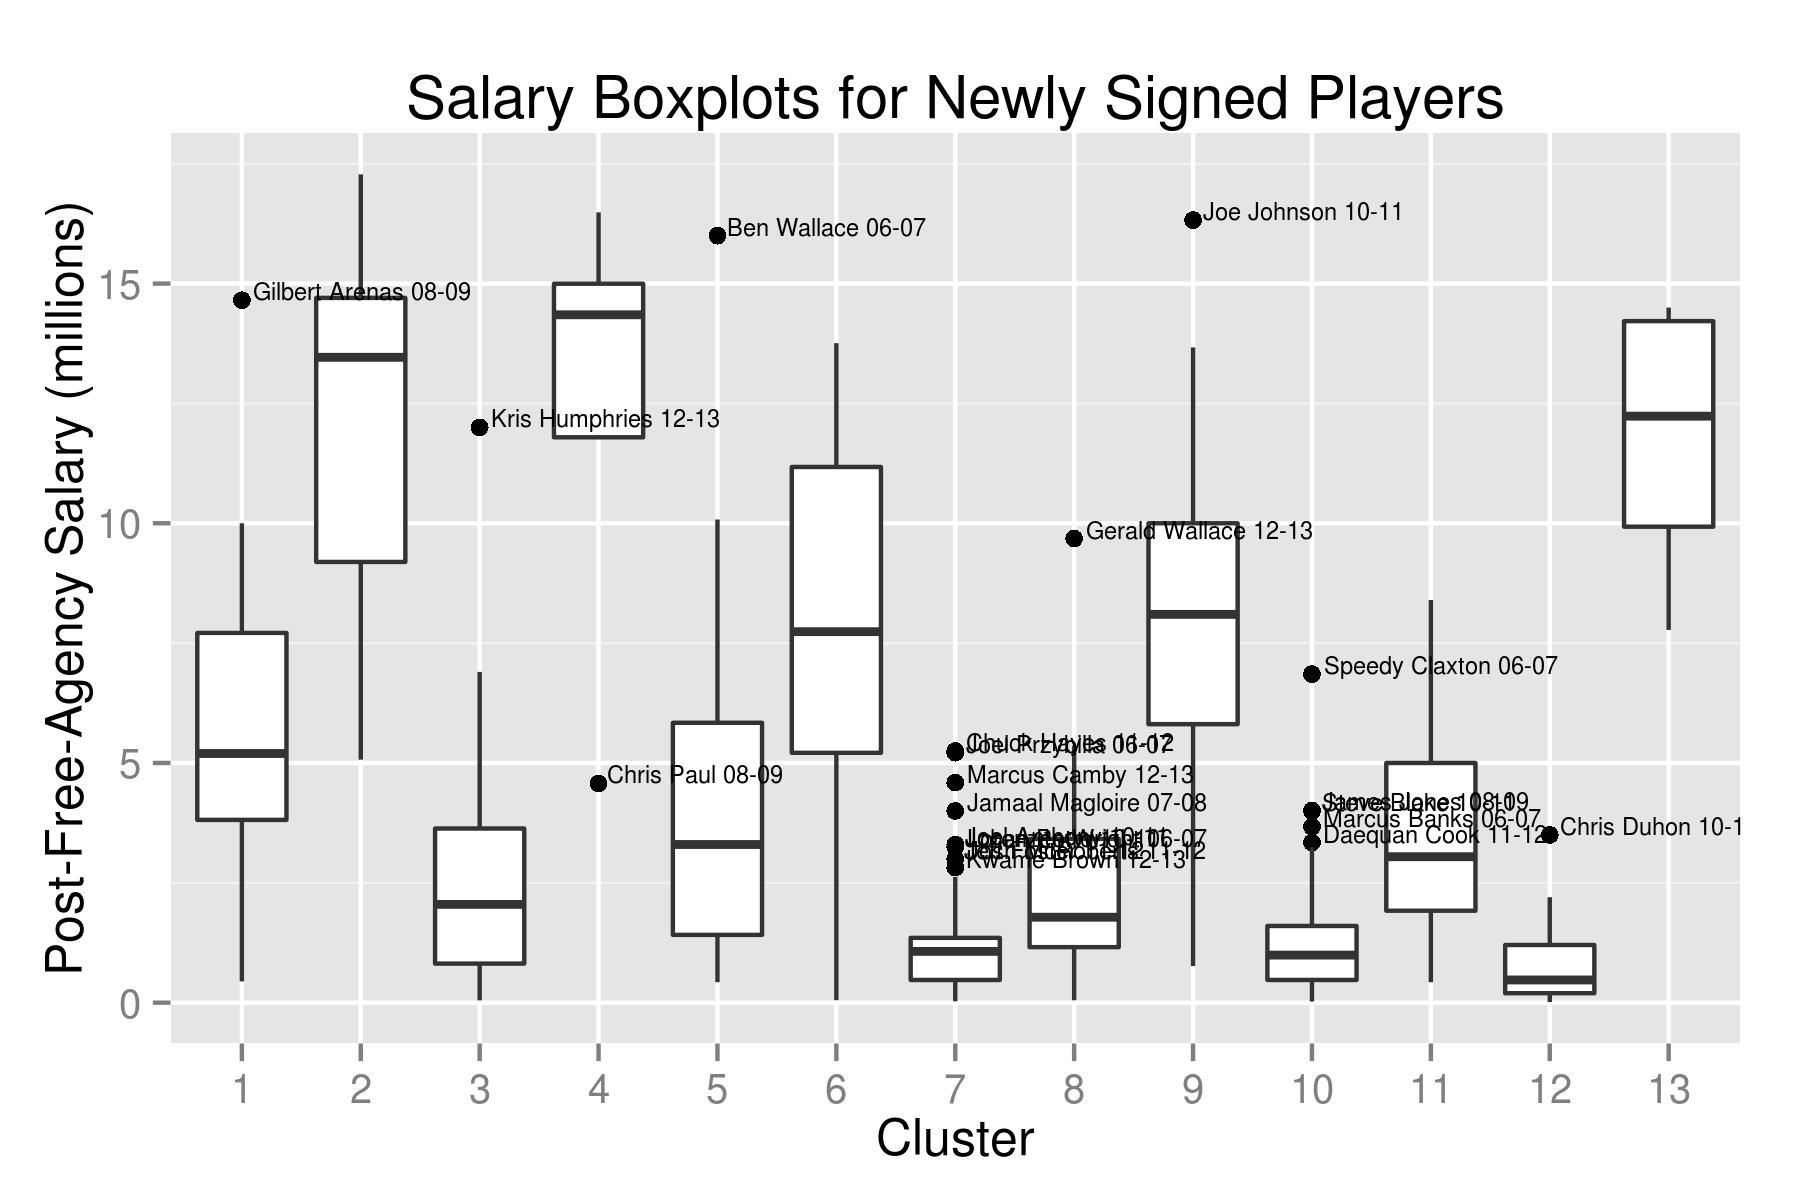
\includegraphics[width=0.8\textwidth]{hw-kmeans-pca.jpeg}
    \caption{$k$-Means using the Hartigan-Wong method and PCA.}
\end{figure}

\section{Analysis}

From the results above, we can draw a few conclusions, as well as predict salaries for upcoming free agents.

First, from observing the PCA eigenvectors (not shown), we find that the features which provide the most variance in salary are indeed minutes played and points. This simply confirms the intuition that players are paid largely based on skill, and skilled players tend to play more minutes and score more points. This also hints at one of the weaknesses of our analysis: since box score data is heavily offense-oriented, defensive players will not be represented well in our clusterings.

Indeed, if we observe the $k$-Means boxplots, some of the high outliers are defensive players. However, in general, the outliers in the data are players who are/were generally agreed as "overpaid". For example, in Figure 7, Joe Johnson in 2010-11 had a relatively disappointing season despite being paid one of the highest salaries in the NBA. Similarly, Gilbert Arenas in 2008-09 was a famously crushing season for Gilbert and the Wizards, even though he was cashing in tens of millions of dollars.

Similarly, we can observe a few players who are low outliers, meaning they were relatively underpaid despite performing in an exceptional cluster. In Figure 4 and Figure 7, we see Chris Paul making under 5 million a year, despite playing at the level of players who make a median of just under 15 million.

Finally, we evaluate some values for upcoming free agents in 2014:

\begin{center}
\begin{tabular}{|c | c | c | c | c|}
\hline
Player & Current Team & Cluster & Median Salary of Cluster (millions)\\
\hline
\hline
Avery Bradley & Boston Celtics & 1 & 6.427 \\
\hline
Luol Deng & Chicago Bulls & 1 & 6.427 \\
\hline
Aaron Brooks & Denver Nuggets & 11 & 3 \\
\hline
Jordan Hamilton & Houston Rockets & 6 & 1.352 \\
\hline
Lance Stephenson & Indiana Pacers & 9 & 7.147 \\
\hline
Eric Bledsoe & Phoenix Suns & 5 & 13.32 \\
\hline
Kevin Seraphin & Washington Wizards & 12 & 1.137 \\
\hline
Trevor Ariza & Washington Wizards & 1 & 6.427 \\
\hline
\end{tabular}
\end{center}

How accurate are these results? We will find out this offseason.

\section{Bibliography}

\printbibliography

\end{document}

